% lintrans - The linear transformation visualizer
% Copyright (C) 2021-2022 D. Dyson (DoctorDalek1963)

% This program is licensed under GNU GPLv3, available here:
% <https://www.gnu.org/licenses/gpl-3.0.html>

\documentclass[../development.tex]{subfiles}

\begin{document}

\subsubsection{Fixing rendering\label{development:improving-the-gui:fixing-rendering}}

Now that I had the basics of matrix visualization sorted, I wanted to make the GUI and UX better. My first step was overhauling the rendering code to make it actually work with rotations of more than $90\degree$.

I narrowed down the issue with PyCharm's debugger and found that the loop in \texttt{VectorGridPlot.draw\_parallel\_lines()} was looping forever if it tried to doing anything outside of the top right quadrant. To fix this, I decided to instead delegate this task of drawing a set of oblique lines to a separate method, and work on that instead.

%: cf05e09e5ebb6ea7a96db8660d0d8de6b946490a
%: src/lintrans/gui/plots/classes.py:203-222

This separation of functionality made designing and debugging this part of the solution much easier. The \texttt{draw\_pair\_of\_oblique\_lines()} method looked like this:

%: cf05e09e5ebb6ea7a96db8660d0d8de6b946490a
%: src/lintrans/gui/plots/classes.py:224-283

To illustrate what this code is doing, I'll use a diagram.

\begin{figure}[H]
	\hspace{0.005\linewidth}
	\centering
	\begin{minipage}{0.48\linewidth}
		\centering
		\begin{figure}[H]
			\centering
			\resizebox{\linewidth}{!}{%
				\begin{tikzpicture}[
					% Style code taken from https://tex.stackexchange.com/questions/123760/draw-crosses-in-tikz#124064
					cross/.style={
						cross out, draw,
						minimum size=2*(#1-\pgflinewidth),
						inner sep=0pt, outer sep=0pt
					},
					cross/.default={5pt}
				]
					% Draw the grid
					\draw [step=1cm,gray,very thin] (-4.9,-4.9) grid (4.9,4.9);
					\draw (-5,0) -- (5,0);
					\draw (0,-5) -- (0,5);

					% Draw the box with dashed extensions
					\draw [dashed] (-4.9,2.8) -- (4.9,2.8);
					\draw [dashed] (-4.9,-2.8) -- (4.9,-2.8);
					\draw [dashed] (-3.2,-4.9) -- (-3.2,4.9);
					\draw [dashed] (3.2,-4.9) -- (3.2,4.9);

					\draw [red,thick] (-3.2,2.8) rectangle (3.2,-2.8);

					% Draw the oblique lines
					\draw [blue,thick] (-1.6,4.9) -- (4.9,3.2);
					\draw [green,thick] (2.1,4.9) -- (-3.3,-4.9);

					% Mark the intersection points
					\draw (0.94286,2.8) node [cross] {};
					\draw (-2.14286,-2.8) node [cross] {};
				\end{tikzpicture}
			}
			\caption{Two example lines and the viewport box}
			\label{tikz:development:cf05e09e5ebb6ea7a96db8660d0d8de6b946490a:lines-and-viewport}
		\end{figure}
	\end{minipage}%
	\hspace{0.015\linewidth}
	\begin{minipage}{0.48\linewidth}
		\centering
		\begin{figure}[H]
			\centering
			\includegraphics[width=\linewidth]{development/cf05e09e5ebb6ea7a96db8660d0d8de6b946490a/gui.png}
			\caption{A demonstration of the new oblique lines system.}
			\label{fig:development:cf05e09e5ebb6ea7a96db8660d0d8de6b946490a:gui.png}
		\end{figure}
	\end{minipage}
	\hspace{0.005\linewidth}
	\vspace{-1em}
\end{figure}

The red box represents the viewport of the GUI. The dashed lines represent the extensions of the red box. For a given line we want to draw, we first want to find where it intersects these orthogonal lines. Any oblique line will intersect each of these lines exactly once. This is what the \texttt{myi}, \texttt{mmyi}, \texttt{mxi}, and \texttt{mmxi} variables represent. The value of \texttt{myi} is the $x$ value where the line intersects the maximum $y$ line, for example.

In the case of the blue line, all 4 intersection points are outside the bounds of the box, whereas the green line intersects with the box, as shown with the crosses. We use a list comprehension over a list of ternaries to get the \texttt{points} list. This list contains 0 or 2 coordinates, and we may or may not draw a line accordingly.

That's how the \texttt{draw\_oblique\_line()} method works, and the \texttt{draw\_pair\_of\_oblique\_lines()} method just calls it with positive and negative values of $c$.

\subsubsection{Adding vector arrowheads\label{development:improving-the-gui:adding-vector-arrowheads}}

\begin{figure}[H]
	\hspace{0.005\linewidth}
	\centering
	\begin{minipage}{0.40\linewidth}
		\centering
		\begin{figure}[H]
			\centering
			\resizebox{\linewidth}{!}{%
				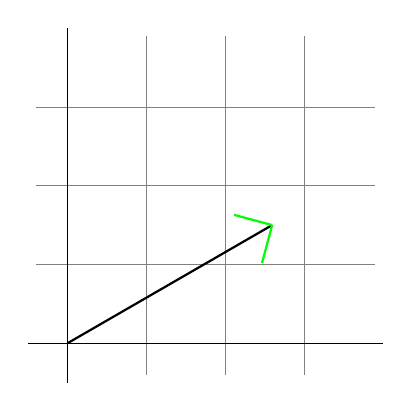
\begin{tikzpicture}
					% Draw the grid
					\draw [step=1cm,gray,very thin] (-0.4,-0.4) grid (3.9,3.9);
					\draw (-0.5,0) -- (4,0);
					\draw (0,-0.5) -- (0,4);

					% Draw the line
					\draw [thick] (0,0) -- (30:3);

					% Draw the arrowheads
					\draw [green,thick] (30:3) -- +(165:0.5);
					\draw [green,thick] (30:3) -- +(255:0.5);
				\end{tikzpicture}
			}
			\caption{An example of a vector with the arrowheads highlighted in green}
			\label{tikz:development:improving-the-gui:adding-vector-arrowheads}
		\end{figure}
	\end{minipage}%
	\hspace{0.015\linewidth}
	\begin{minipage}{0.56\linewidth}\setspacing
		Now that I had a good renderer, I wanted to add arrowheads to the vectors to make them easier to see. They were already thicker than the gridlines, but adding arrowheads like in the 3blue1brown series would make them much easier to see. Unfortunately, I couldn't work out how to do this.

		I wanted a function that would take a coordinate, treat it as a unit vector, and draw lines at $45\degree$ angles at the tip. This wasn't how I was conceptualising the problem at the time and because of that, I couldn't work out how to solve this problem. I could create this $45\degree$ lines in the top right quadrant, but none of my possible solutions worked for any arbitrary point.

		So I started googling and found a very nice algorithm on \texttt{csharphelper.com}\cite{csharphelper-arrowheads}, which I adapted for Python.
	\end{minipage}
	\hspace{0.005\linewidth}
	\vspace{-1em}
\end{figure}

%: 5373b1ad8040f6726147cccea523c0570251cf67
%: src/lintrans/gui/plots/widgets.py:52-86

As the comments suggest, we get the $x$ and $y$ components of the normalised vector, and then do some magic with a chosen length and get some distance values, and then draw those lines. I don't really understand how this code works, but I'm happy that it does. All we have to do is call \texttt{draw\_vector\_arrowheads()} from \texttt{paintEvent()}.

\begin{figure}[H]
	\centering
	\includegraphics[width=0.8\linewidth]{development/5373b1ad8040f6726147cccea523c0570251cf67/gui.png}
	\caption{An example of the $i$ and $j$ vectors with arrowheads}
	\label{fig:development:5373b1ad8040f6726147cccea523c0570251cf67:gui.png}
\end{figure}

\subsubsection{Implementing zoom\label{development:improving-the-gui:implementing-zoom}}

The next thing I wanted to do was add the ability to zoom in and out of the viewport, and I wanted a button to reset the zoom level as well. I added a \texttt{default\_grid\_spacing} class attribute in \texttt{BackgroundPlot} and used that as the \texttt{grid\_spacing} instance attribute in \texttt{\_\_init\_\_()}.

%: d944e86e1d0fdc2c4be4d63479bc6bc3a31568ef
%: src/lintrans/gui/plots/classes.py:27-47

The reset button in \texttt{LintransMainWindow} simply sets \texttt{plot.grid\_spacing} to the default.

To actually allow for zooming, I had to implement the \texttt{wheelEvent()} method in \texttt{BackgroundPlot} to listen for mouse wheel events. After reading through the docs for the \texttt{QWheelEvent} class\cite{qt5-docs-qwheelevent}, I learned how to handle this event.

%: d944e86e1d0fdc2c4be4d63479bc6bc3a31568ef
%: src/lintrans/gui/plots/classes.py:119-128

All we do is get the amount that the user scrolled and add that to the current spacing, taking the max with 1, which acts as a minimum grid spacing. We need to use \texttt{degrees.y()} on line 125 because Qt5 allows for mice that can scroll in the $x$ and $y$ directions, and we only want the $y$ component. Line 127 marks the event as accepted so that the parent widget doesn't try to act on it.

\begin{figure}[H]
	\hspace{0.005\linewidth}
	\centering
	\begin{minipage}{0.48\linewidth}
		\centering
		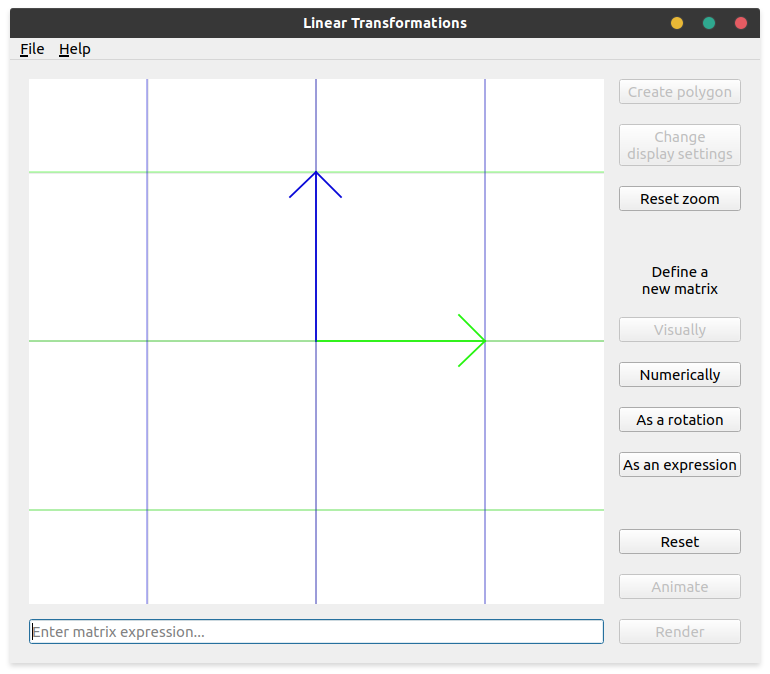
\includegraphics[width=\linewidth]{development/d944e86e1d0fdc2c4be4d63479bc6bc3a31568ef/zoomed-in.png}
		\caption{The GUI zoomed in a bit}
		\label{fig:development:d944e86e1d0fdc2c4be4d63479bc6bc3a31568ef:zoomed-in.png}
	\end{minipage}\hspace{0.015\linewidth}
	\begin{minipage}{0.48\linewidth}
		\centering
		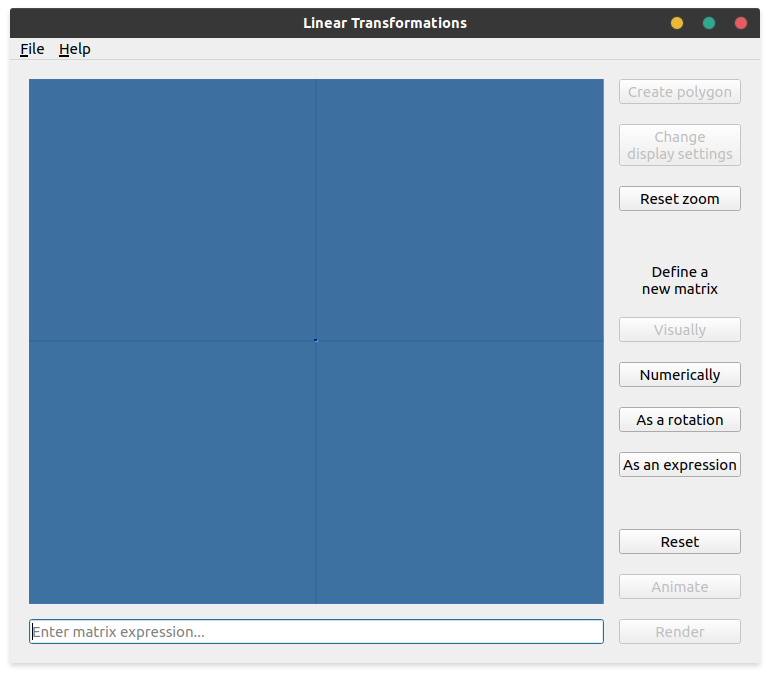
\includegraphics[width=\linewidth]{development/d944e86e1d0fdc2c4be4d63479bc6bc3a31568ef/max-zoomed-out.png}
		\caption{The GUI zoomed out as far as possible}
		\label{fig:development:d944e86e1d0fdc2c4be4d63479bc6bc3a31568ef:max-zoomed-out.png}
	\end{minipage}
	\hspace{0.005\linewidth}
	\vspace{-1em}
\end{figure}

There are two things I don't like here. Firstly, the minimum grid spacing is too small. The user can zoom out too far. Secondly, the arrowheads are too big in figure~\ref{fig:development:d944e86e1d0fdc2c4be4d63479bc6bc3a31568ef:zoomed-in.png}.

The first problem is minor and won't be fixed for quite a while, but I fixed the second problem quite quickly.

We want the arrowhead length to not just be 0.15, but to scale with the zoom level (the ratio between default grid spacing and current spacing).

This creates a slight issue when zoomed out all the way, because the arrowheads are then far larger than the vectors themselves, so we take the minimum of the scaled length and the vector length.

I factored out the default arrowhead length into the \texttt{arrowhead\_length} instance attribute and initialize it in \texttt{\_\_init\_\_()}.

%: 3d19a003368ae992ebb60049685bb04fde0836b5
%: src/lintrans/gui/plots/widgets.py:68-76

This code results in arrowheads that stay the same length unless the user is zoomed out basically as far as possible.

\begin{figure}[H]
	\centering
	\includegraphics[width=0.8\linewidth]{development/3d19a003368ae992ebb60049685bb04fde0836b5/gui.png}
	\caption{The arrowheads adjusted for zoom level}
	\label{fig:development:3d19a003368ae992ebb60049685bb04fde0836b5:gui.png}
\end{figure}

\subsubsection{Animation blocks zooming\label{development:improving-the-gui:animation-blocks-zooming}}

The biggest problem with this new zoom feature is that when animating between matrices, the user is unable to zoom. This is because when \texttt{LintransMainWindow.animate\_expression()} is called, it uses Python's standard library \texttt{time.sleep()} function to delay each frame, which prevents Qt from handling user interaction while we're animating. This was a problem.

I did some googling and found a helpful post on StackOverflow\cite{so-update-window-in-pyqt5} that gave me a nice solution. The user \texttt{ekhumoro} used the functions \texttt{QApplication.processEvents()} and \texttt{QThread.msleep()} to solve the problem, and I used these functions in my own app, with much success.

After reading \enquote{The Event System} in the Qt5 documentation\cite{qt5-docs-event-system}, I learned that Qt5 uses an event loop, a lot like JavaScript. This means that events are scheduled to be executed on the next pass of the event loop. I also read the documentation for the \texttt{repaint()} and \texttt{update()} methods on the \texttt{QWidget} class\cite{qt5-docs-qwidget-repaint,qt5-docs-qwidget-update} and decided that it would be better to just queue a repaint by calling \texttt{update()} on the plot rather than immediately repaint with \texttt{repaint()}, and then call \texttt{QApplication.processEvents()} to process the pending events on the main thread. This is a nicer way of repainting, which reduces potential flickering issues, and using \texttt{QThread.msleep()} allows for asynchronous processing and therefore non-blocking animation.

\subsubsection{Rank 1 transformations\label{development:improving-the-gui:rank-1-transformations}}

The rank of a matrix is the dimension of its column space. This is the dimension of the span of its columns, which is to say the dimension of the output space. The rank of a matrix must be less than or equal to the dimension of the matrix, so we only need to worry about ranks 0, 1, and 2. There is only one rank 0 matrix, which is the $\mathbf{0}$ matrix itself. I've already covered this case by just not drawing any transformed grid lines.

Rank 2 matrices encompass most 2D matrices, and I've already covered this case in \S\ref{development:visualizing-matrices:drawing-the-transformed-grid} and \S\ref{development:improving-the-gui:fixing-rendering}. A rank 1 matrix collapses all of 2D space onto a single line, so for this type of matrix, we should just draw this line.

This code is in \texttt{VectorGridPlot.draw\_parallel\_lines()}. We assemble the matrix $\begin{pmatrix}\text{\texttt{vector\_x}} & \text{\texttt{point\_x}}\\ \text{\texttt{vector\_y}} & \text{\texttt{point\_y}}\end{pmatrix}$ (which is actually the matrix used to create the transformation we're trying to render lines for) and use this matrix to check determinant and rank.

%: 677b38c87bb6722b16aaf35058cf3cef66e43c21
%: src/lintrans/gui/plots/classes.py:177-192

Additionally, there was a bug with animating these determinant 0 matrices, since we try to scale the determinant through the animation, as documented in \S\ref{development:visualizing-matrices:preserving-determinants}, but when the determinant is 0, this causes issues. To fix this, we just check the \texttt{det\_target} variable in \texttt{LintransMainWindow.animate\_expression} and if it's 0, we use the non-scaled version of the matrix.

%: b889b686d997c2b64124bee786bccba3fc4f6b08
%: src/lintrans/gui/main_window.py:307-315

\subsubsection{Matrices that are too big\label{development:improving-the-gui:matrices-that-are-too-big}}

One of my friends was playing around with the prototype and she discovered a bug. When trying to render really big matrices, we can get errors like \enquote{\pyinline{OverflowError}\texttt{: argument 3 overflowed: value must be in the range -2147483648 to 2147483647}} because PyQt5 is a wrapper over Qt5, which is a C++ library that uses the C++ \mintinline{C++}{int} type for the \texttt{painter.drawLine()} call. This type is a 32-bit integer. Python can store integers of arbitrary precision, but when PyQt5 calls the underlying C++ library code, this gets cast to a C++ \mintinline{C++}{int} and we can get an \pyinline{OverflowError}.

This isn't a problem with the gridlines, because we only draw them inside the viewport, as discussed in \S\ref{development:improving-the-gui:fixing-rendering}, and these calculations all happen in Python, so integer precision is not a concern. However, when drawing the basis vectors, we just draw them directly, so we'll have to check that they're within the limit.

I'd previously created a \texttt{LintransMainWindow.show\_error\_message()} method for telling the user when they try to take the inverse of a singular matrix\footnote{This commit didn't get a standalone section in this write-up because it was so small}.

%: 0f699dd95b6431e95b2311dcb03e7af49c19613f
%: src/lintrans/gui/main_window.py:378-396

I then created the \texttt{is\_matrix\_too\_big()} method to just check that the elements of the matrix are within the desired bounds. If it returns \pyinline{True} when we try to render or animate, then we call \texttt{show\_error\_message()}.

%: 4682a7b225747cfd77aca0fe3abcdd1397b7c5dd
%: src/lintrans/gui/main_window.py:407-421

\subsubsection{Creating the \texttt{DefineVisuallyDialog}\label{development:improving-the-gui:creating-the-DefineVisuallyDialog}}

Next, I wanted to allow the user to define a matrix visually by dragging the basis vectors. To do this, I obviously needed a new \texttt{DefineDialog} subclass for it.

%: 16ca0229aab73b3f4a8fe752dee3608f3ed6ead5
%: src/lintrans/gui/dialogs/define_new_matrix.py:135-189

This \texttt{DefineVisuallyDialog} class just implements the normal methods needed for a \texttt{DefineDialog} and has a \texttt{plot} attribute to handle drawing graphics and handling mouse movement. After creating the \texttt{DefineVisuallyWidget} as a skeleton and doing some more research in the Qt5 docs\cite{qt5-docs-qwidget-mousemoveevent}, I renamed the \texttt{trans\_coords()} methods to \texttt{canvas\_coords()} to make the intent more clear, and created a \texttt{grid\_coords()} method.

%: 417aea6555029b049c470faff18df29f064f6101
%: src/lintrans/gui/plots/classes.py:85-94

I then needed to implement the methods to handle mouse movement in the \texttt{DefineVisuallyWidget} class. Thankfully, Ross Wilson, the person who helped me learn about the \texttt{QWidget.paintEvent()} method in \S\ref{development:visualizing-matrices:asking-strangers-on-the-internet-for-help}, also wrote an example of draggable points\cite{gitlab-custom-widgets-ijvectors.py}. In my post, I had explained that I needed draggable points on my canvas, and Ross was helpful enough to create an example in their own time. I probably could've worked it out myself eventually, but this example allowed me to learn a lot quicker.

%: 417aea6555029b049c470faff18df29f064f6101
%: src/lintrans/gui/plots/widgets.py:56-121

This snippet has the line \enquote{\pyinline{self.setMouseTracking(True)}} commented out. This line was in the example, but it turns out that I don't want it. Mouse tracking means that a widget will receive a \texttt{QMouseEvent} every time the mouse moves. But if it's disabled (the default), then the widget will only receive a \texttt{QMouseEvent} for mouse movement when a button is held down at the same time.

I've also left in some print statements on lines 116 and 117. These small oversights are there because I just forgot to remove them before I committed these changes. They were removed 3 commits later.

\subsubsection{Fixing a division by zero bug\label{development:improving-the-gui:fixing-a-division-by-zero-bug}}

When drawing the rank line for a determinant 0, rank 1 matrix, we can encounter a division by zero error. I'm sure this originally manifested in a crash with a \pyinline{ZeroDivisionError} at runtime, but now I can only get a \pyinline{RuntimeWarning} when running the old code from commit \texttt{16ca0229aab73b3f4a8fe752dee3608f3ed6ead5}. Whether it crashes or just warns the user, there is a division by zero bug when trying to render $\begin{pmatrix}k & 0\\ 0 & 0\end{pmatrix}$ or $\begin{pmatrix}0 & 0\\ 0 & k\end{pmatrix}$. To fix this, I just handled those cases separately in \pyinline{VectorGridPlot.draw_parallel_lines()}.

%: 40bee6461d477a5c767ed132359cd511c0051e3b
%: src/lintrans/gui/plots/classes.py:196-207

\subsubsection{Implementing transitional animation\label{development:improving-the-gui:implementing-transitional-animation}}

Currently, all animation animates from $\mathbf{I}$ to the target matrix $\mathbf{T}$. This means it resets the plot at the start. I eventually want an applicative animation system, where the matrix in the box is applied to the current scene. But I also want an option for a transitional animation, where the program animates from the start matrix $\mathbf{S}$ to the target matrix $\mathbf{T}$, and this seems easier to implement, so I'll do it first.

In \texttt{LintransMainWindow}, I created a new method called \texttt{animate\_between\_matrices()} and I call it from \texttt{animate\_expression()}. The maths for smoothening determinants in \S\ref{development:visualizing-matrices:preserving-determinants} assumed the starting matrix had a determinant of 1, but when using transitional animation, this may not always be true.

If we let $\mathbf{S}$ be the starting matrix, and $\mathbf{A}$ be the matrix from the first stage of calculation as specified in \S\ref{development:visualizing-matrices:preserving-determinants}, then we want a $c$ such that $\det(c\mathbf{A}) = \det(\mathbf{S})$, so we get $c = \sqrt{\left|\dfrac{\det(\mathbf{S})}{\det(\mathbf{A})}\right|}$ by the identity $\det(c\mathbf{A}) = c^2 \det(\mathbf{A})$.

Following the same logic as in \S\ref{development:visualizing-matrices:preserving-determinants}, we can let $\mathbf{B} = c\mathbf{A}$ and then scale it by $d$ to get the same determinant as the target matrix $\mathbf{T}$ and find that $d = \sqrt{\left|\dfrac{\det(\mathbf{T})}{\det(\mathbf{B})}\right|}$. Unlike previously, $\det(\mathbf{B})$ could be any scalar, so we can't simplify our expression for $d$.

We then scale this with our \texttt{proportion} variable $p$ to get a scalar $s = 1 + p\left(\sqrt{\left|\dfrac{\det(\mathbf{T})}{\det(\mathbf{B})}\right|} - 1\right)$ and render $\mathbf{C} = s\mathbf{B}$ on each frame.

In code, that looks like this:

%: 4017b84fbce67d8e041bc9ce84cefcb0b6e65e1f
%: src/lintrans/gui/main_window.py:275-356

This change results in an animation system that will transition from the current matrix to whatever the user types into the input box.

\subsubsection{Allowing for sequential animation with commas\label{development:improving-the-gui:allowing-for-sequential-animation-with-commas}}

Applicative animation has two main forms. There's the version where a standard matrix expression gets applied to the current scene, and the kind where the user defines a sequence of matrices and we animate through the sequence, applying one at a time. Both of these are referenced in success criterion \ref{success-criterion:applicative-animation}.

I want the user to be able to decide if they want applicative animation or transitional animation, so I'll need to create some form of display settings. However, transitional animation doesn't make much sense for sequential animation\footnote{I have since changed my thoughts on this, and I allowed sequential transitional animation much later, in commit \texttt{41907b81661f3878e435b794d9d719491ef14237}}, so I can implement this now.

Applicative animation is just animating from the matrix $\mathbf{C}$ representing the current scene to the composition $\mathbf{TC}$ with the target matrix $\mathbf{T}$.

We use $\mathbf{TC}$ instead of $\mathbf{CT}$ because matrix multiplication can be thought of as applying successive transformations from right to left. $\mathbf{TC}$ is the same as starting with the identity $\mathbf{I}$, applying $\mathbf{C}$ (to get to the current scene), and then applying $\mathbf{T}$.

Doing this in code is very simple. We just split the expression on commas, and then apply each sub-expression to the current scene one by one, pausing on each comma.

%: 60584d2559cacbf23479a1bebbb986a800a32331
%: src/lintrans/gui/main_window.py:284-325

We're deliberately not checking if the sub-expressions are valid here. We would normally validate the expression in \texttt{LintransMainWindow.update\_render\_buttons()} and only allow the user to render or animate an expression if it's valid. Now we have to check all the sub-expressions if the expression contains commas. Additionally, we can only animate these expressions with commas in them, so rendering should be disabled when the expression contains commas.

Compare the old code to the new code:

%: 4017b84fbce67d8e041bc9ce84cefcb0b6e65e1f
%: src/lintrans/gui/main_window.py:243-247

%: 60584d2559cacbf23479a1bebbb986a800a32331
%: src/lintrans/gui/main_window.py:243-256

\end{document}
